\documentclass[3p,sort&compress,11pt,fleqn,review]{elsarticle}
\bibliographystyle{elsarticle-num-names}
\usepackage{amsmath,amsfonts,amssymb,siunitx,float,subcaption,setspace,booktabs,diagbox,bm,tikz,structmech,mathtools,tikz-3dplot,pgfplots,url,mathrsfs}
\usepackage{algorithm}
\usepackage{algpseudocode}
\usepackage{lineno}
%\usepackage{easyReview}
\usetikzlibrary{shapes.geometric,backgrounds}
\pgfplotsset{compat=1.8}
\journal{}
\newcommand*{\add}[1]{#1}
\newcommand*{\mb}[1]{\bm{#1}}
\newcommand*{\mT}{\mathrm{T}}
\newcommand*{\md}[1]{\mathrm{d}#1}
\newcommand*{\mdd}[1]{\mathrm{d}^2#1}
\newcommand*{\eqsref}[1]{Eq.~(\ref{#1})}
\newcommand*{\figref}[1]{Fig.~\ref{#1}}
\newcommand*{\tabref}[1]{Table~\ref{#1}}
\newcommand*{\algoref}[1]{Algorithm~\ref{#1}}
\newcommand*{\secref}[1]{\S~\ref{#1}}
\newcommand*{\diag}[1]{\text{diag}\left(#1\right)}
\newcommand*{\sign}[1]{\text{sign}\left(#1\right)}
\newcommand*{\dev}[1]{\text{dev}\left(#1\right)}
\newcommand*{\tr}[1]{\text{trace}\left(#1\right)}
\newcommand*{\ddfrac}[2]{\dfrac{\md{#1}}{\md{#2}}}
\newcommand*{\pdfrac}[2]{\dfrac{\partial{#1}}{\partial{#2}}}
\newcommand{\bsigma}{\mb{\sigma}}
\newcommand{\bvarepsilon}{\mb{\varepsilon}}
\newcommand{\beeta}{\mb{\eta}}
\newcommand{\bn}{\mb{n}}
\newcommand{\balpha}{\mb{\alpha}}
\newcommand{\bbeta}{\mb{\beta}}
\newcommand{\bgamma}{\mb{\gamma}}
\newcommand{\bzeta}{\mb{\zeta}}
\newcommand{\bq}{\mb{q}}
\newcommand{\bs}{\mb{s}}
\newcommand{\bc}{\mb{c}}
\newcommand{\be}{\mb{e}}
\newcommand{\bv}{\mb{v}}
\newcommand{\bd}{\mb{d}}
\DeclarePairedDelimiter\abs{\lvert}{\rvert}
\DeclarePairedDelimiter\norm{\lVert}{\rVert}
\makeatletter
\let\oldabs\abs
\def\abs{\@ifstar{\oldabs}{\oldabs*}}
\let\oldnorm\norm
\def\norm{\@ifstar{\oldnorm}{\oldnorm*}}
\newenvironment{breakablealgorithm}
{\begin{center}
\refstepcounter{algorithm}
\hrule height.8pt depth0pt \kern2pt
\renewcommand{\caption}[2][\relax]{
{\raggedright\textbf{\ALG@name~\thealgorithm} ##2\par}
\ifx\relax##1\relax
\addcontentsline{loa}{algorithm}{\protect\numberline{\thealgorithm}##2}
\else
\addcontentsline{loa}{algorithm}{\protect\numberline{\thealgorithm}##1}
\fi
\kern2pt\hrule\kern2pt
}}{\kern2pt\hrule\relax
\end{center}}
\begin{document}
\linenumbers
\begin{abstract}
    \begin{linenumbers}
        This study focuses on the analytical identification and quantification of one type of spurious responses in the context of response history analysis. The spurious response is caused by linear interpolation of input loads. Through analytical derivation and numerical simulations, it is shown that the identified spurious response is fully caused by interpolation and can significantly affect both damping and inertial forces. Furthermore, the spurious response is not bounded, thus, resistance-based designs could potentially be non-conservative. The findings are applicable to (non-)linear MDOF systems. To address this issue and improve the quality of numerical results, remedies and recommendations are proposed.
    \end{linenumbers}
\end{abstract}
\begin{keyword}
    response history analysis\sep
    spurious structural response\sep
    time integration\sep
    digital signal processing\sep
    dynamics
\end{keyword}
\begin{frontmatter}
    \title{Subloading Surface Model}
    \author[add1]{Theodore~L.~Chang\corref{tlc}}\ead{tlcfem@gmail.com}
    \cortext[tlc]{corresponding author}
    \address[add1]{IRIS Adlershof, Humboldt-Universität zu Berlin, Berlin, Germany, 12489.}
\end{frontmatter}
\section{Introduction}
The conventional plasticity theory adopts the concept of yield/loading surface \citep[see, e.g.,][]{Lemaitre1990,Simo1998} to describe the onset of plastic deformation.
The surface encloses a region where the material is elastic, and once the stress state reaches the surface, plastic deformation occurs.
Because of this clear distinction between elastic and plastic states, the corresponding stiffness is often discontinuous when transiting from elastic to plastic states.
Although such a discontinuity is not physically sound, this is often not a concern for most models as the capability of capturing more accurate cyclic responses (and/or other objectives) is often more important, especially for metals.
To this end, models employ advanced/modified kinematic hardening rules enriched with various types of rate control and hardening activation/deactivation, such as Ohno's modifications \citep[see, e.g.,][]{Ohno1982,Ohno1993,Ohno2021} and Yoshida's modification \citep{Yoshida2002}, based on the famous Armstrong--Frederick rule \citep{Frederick2007} and its multiplicative version, see a comprehensive review by \citet{Chaboche2008}, have been proposed.
However, models of this kind often present decent cyclic responses under two--sided cyclic loading but are \emph{`incapable of describing the \textnormal{(general, including one--sided and small cycles)} cyclic loading behaviour'} \citep[][pg. 282]{Hashiguchi2023} due to the existence of the elastic region, regardless of large or small \citep{Dafalias1977}.
As an alternative to the conventional macroscopic approach, the polycrystalline models \citep[see, e.g.,][]{Beyerlein2018} employ a microscopic approach to describe the plastic deformation, which is able to capture the cyclic behaviour more accurately.
However, the corresponding computational cost is high as often fine microstructural details are required.

Within the same macroscopic framework, on the contrary, the subloading surface model offers a quite unique approach that is different from the conventional framework.
The initial proposal of the subloading surface model can be dated back to the work by \citet{Hashiguchi1980}.
The model is later extended \citep{Hashiguchi1989} to include an elastic core, which enables the model to describe more versatile cyclic responses.
Over the decades of development, it has been widely adopted in various applications, to name a few recent endeavours, see the work by \citet{Maranha2016,Xiong2018,Anjiki2021,Yamakawa2021,Yamakawa2022,Lu2023}.
The comprehensive review of the subloading surface model and its extended version can be found in the recent review papers by \citet{Hashiguchi2023a} and \citet{Hashiguchi2024}.
Meanwhile, the classification and overview of plasticity models is summarised and well documented in the monograph by \citet[see][\S~10.2]{Hashiguchi2023}.
Interested readers are referred to these references for more detailed information.

The (extended) subloading surface model possesses many advantages over conventional plasticity models.
The most notable one is that it provides a smooth transition between elastic and plastic states, implying the tangent stiffness is continuous under all loading conditions.
Such a continuity is more realistic and tends to be beneficial not only for static analyses, but also for other applications such as damping formulation, for example, a stiffness proportional damping based on the tangent stiffness matrix would now result in a continuous damping matrix, thus, a continuous damping force.
Furthermore, due to the introduction of the elastic core in the extended version, it is much more capable of describing ratcheting behaviour under cyclic loading, which cannot be well captured by conventional models that incorporate a pure elastic region.

The choice of internal history variables in the existing formulation bears a clear and straightforward physical implication.
However, their evolution rules \citep[see, e.g.,][]{Hashiguchi2024} appear to be somewhat cumbersome and not very intuitive.
Due to the same reason, the corresponding numerical implementation \citep[see, e.g.,][]{Fincato2017,Anjiki2019,Anjiki2021} involves a local system possessing a significant size (around \num{20} for 3D models).
Thus, it appears to be less efficient and robust.
In this work, we focus on the following three tasks:
\begin{enumerate}
    \item revise the definition(s) and the corresponding evolution rule(s) of some key internal history variables to make them concise and intuitive both analytically and numerically;
    \item propose a concise and universal loading/unloading criterion that is cheap to evaluate and can be easily implemented;
    \item improve numerical stability by discussing and choosing more numerical friendly functions for the evolution rules.
\end{enumerate}
As a showcase, a reference algorithm is also presented which adopts the von Mises framework that is suitable for metals.

The paper is organized as follows.
The original formulation of the (extended) subloading surface model is briefly reviewed in \secref{sec:subloading}.
Based on which, a revised formulation with improved evolution rules and loading/unloading criterion is proposed in \secref{sec:revised}.
A reference implementation for von Mises materials is presented thereafter.
Numerical analyses cover the comparison between the conventional and the proposed (un)loading criterion and the accuracy analysis of the proposed algorithm.
\section{Subloading Surface Model}
In this section, the framework of the (extended) subloading surface model is briefly reviewed and summarised.
\subsection{The Subloading Surface}
The conventional plasticity models often adopt the concept of the yield surface, denoted by $f\left(\bsigma,\cdots\right)$, which defines the frontier of plasticity.
For example,
\begin{gather}
    f=\norm{\beeta}-F,
\end{gather}
in which $\beeta$ is known as the shifted stress, $F$ characterises the size of the surface and could evolve with the development of plasticity.
Within the yield surface, the material is elastic, while plasticity would develop once the stress state reaches the yield surface.
Thus any admissible state shall satisfy the inequality $f\leqslant0$.

The original proposal of the subloading surface model introduces the concept of the normal yield ratio, denoted by $z$ in this work, which effectively scales the yield surface $f$ down by a factor of $z$, the new surface is call the subloading surface $f_s$ and it is concentric with the yield surface $f$.
\begin{gather}
    f_s=\norm{\beeta}-zF.
\end{gather}
The normal yield ratio $0\leqslant{}z\leqslant{}1$ shall be updated in a manner such that $f_s=0$ is enforced not only for plastic loading but also for elastic unloading.
With such a construct, any given stress state would always lie on the subloading surface.

The main shortcoming of the original subloading surface model is the excessive strain accumulation under cyclic loading.
To address this issue, the extended subloading surface model introduces the concept of the elastic core.
An additional internal field, denoted by $\bc$, is adopted to define the elastic core surface, which is concentric with the yield surface (centred at the back stress $\balpha$).

The subloading surface is then pulled from the original centre $\balpha$ towards $\bc$ by a certain amount governed by the normal yield ratio $z$.
\begin{figure}[htb]
    \centering\footnotesize
    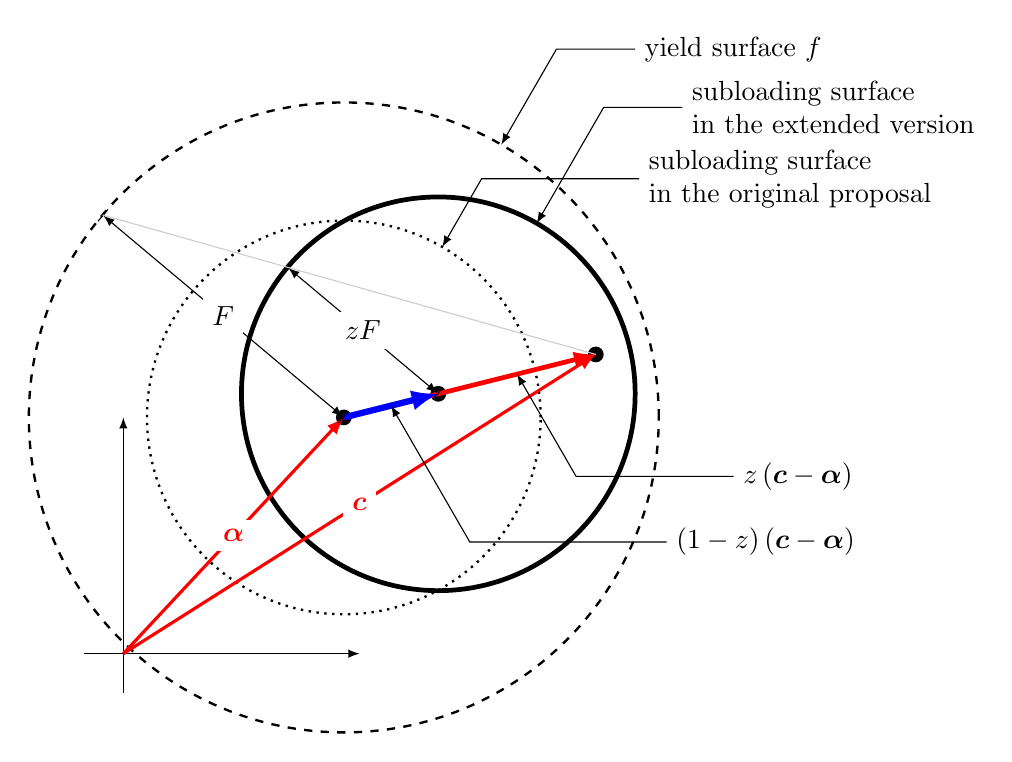
\begin{tikzpicture}[>=latex]
        \newcommand{\Ax}{2.8}
        \newcommand{\Ay}{3}
        \newcommand{\Bx}{6}
        \newcommand{\By}{3.8}
        \pgfmathsetmacro{\RR}{sqrt((\Bx-\Ax)^2+(\By-\Ay)^2)}
        \draw[->](-.5,0)--(3,0);
        \draw[->](0,-.5)--(0,3);
        \coordinate(A)at(\Ax,\Ay);
        \coordinate(B)at(\Bx,\By);
        \coordinate(C)at($(A)!0.375!(B)$);
        \node[fill=black,circle,inner sep=0,minimum size=2mm]at(A){};
        \node[fill=black,circle,inner sep=0,minimum size=2mm]at(B){};
        \node[fill=black,circle,inner sep=0,minimum size=2mm]at(C){};
        \draw[dashed,draw,line width=.3mm](A)circle(4cm);
        \draw[dotted,draw,line width=.3mm](A)circle(2.5cm);
        \draw[draw,line width=.6mm](C)circle(2.5cm);
        \draw[->,red,line width=.4mm](0,0)--(A)node[midway,fill=white]{$\balpha$};
        \draw[->,red,line width=.6mm](A)--(B);
        \draw[->,red,line width=.4mm](0,0)--(B)node[midway,fill=white]{$\bc$};
        \draw[->,blue,line width=.8mm](A)--(C);
        \draw[|<->|](A)--++(140:4)node[midway,fill=white]{$F$};
        \draw[|<->|](C)--++(140:2.5)node[midway,fill=white]{$zF$};
        \draw[<-]($(A)+(60:4)$)--++(60:1.4)--++(1,0)node[right,fill=white]{yield surface $f$};
        \draw[<-]($(A)+(60:2.5)$)--++(60:1)--++(2,0)node[right,fill=white,align=left]{subloading surface\\in the original proposal};
        \draw[<-]($(C)+(60:2.5)$)--++(60:1.7)--++(1,0)node[right,fill=white,align=left]{subloading surface\\in the extended version};
        \draw[<-]($(C)!0.5!(B)$)--++(-60:1.5)--++(2,0)node[right,fill=white]{$z\left(\bc-\balpha\right)$};
        \draw[<-]($(A)!0.5!(C)$)--++(-60:2)--++(2.5,0)node[right,fill=white]{$\left(1-z\right)\left(\bc-\balpha\right)$};
        \draw[black!20]($(A)+(140:4)$)--(B);
    \end{tikzpicture}
    \caption{graphical representation of the surfaces used in the subloading surface model}\label{fig:surfaces}
\end{figure}
A graphical illustration is shown in \figref{fig:surfaces}.
By definition, $\bc$ denotes the homothetic centre between $f$ and $f_s$.
Then, according to similarity, the new centre of the subloading surface is $\balpha+\left(1-z\right)\left(\bc-\balpha\right)$, that is $z\balpha+\left(1-z\right)\bc$.
\subsection{A von Mises Material Model}
\subsubsection{Subloading Surface}
\begin{gather}
    f_s=\norm{\beeta}-z\sqrt{\dfrac{2}{3}}\sigma^y.
\end{gather}
In which, $\sigma^y$ denotes the yield stress that evolves with the accumulated plastic strain $q$.
Noting now $\beeta=\dev{\bsigma}-a^y\balpha+\left(z-1\right)\sigma^y\bd$.
\subsubsection{Flow Rule}
Assuming associative plasticity, the flow rule is given by
\begin{gather}\label{eq:subloading_flow}
    \dot{\bvarepsilon^p}=\gamma\pdfrac{f_s}{\bsigma}=\gamma\dfrac{\beeta}{\norm{\beeta}}=\gamma\bn,
\end{gather}
where $\gamma$ denotes the plastic multiplier.
\subsubsection{Evolution Rules}
\paragraph{Accumulated Plastic Strain}
The accumulated plastic strain $q$ simply takes the accumulated magnitude of $\bvarepsilon^p$, thus, its rate form is
\begin{gather}
    \dot{q}=\sqrt{\dfrac{2}{3}}\norm{\dot{\bvarepsilon^p}}=\sqrt{\dfrac{2}{3}}\gamma.
\end{gather}
\paragraph{Isotropic Hardening}
The evolution of $\sigma^y$ depends on $q$, here we adopt general form that combines linear hardening and nonlinear saturation.
\begin{gather}
    \sigma^y=\sigma^i+k_\text{iso}q+\sigma^s_\text{iso}\left(1-e^{-m^s_\text{iso}q}\right),
    \end{gather}
    where $\sigma^i$ is the initial yield stress, $k_\text{iso}$ is the isotropic hardening modulus, $\sigma^s_\text{iso}$ is the saturation stress, and $m^s_\text{iso}$ is the saturation rate.
    \paragraph{Kinematic Hardening}
    The kinematic hardening bound $a^y$ takes a similar form,
    \begin{gather}
        a^y=a^i+k_\text{kin}q+a^s_\text{kin}\left(1-e^{-m^s_\text{kin}q}\right),
    \end{gather}
    where $a^i$ is the initial stress, $k_\text{kin}$ is the kinematic hardening modulus, $a^s_\text{kin}$ is the saturation stress, and $m^s_\text{kin}$ is the saturation rate.
    
    The normalised back stress $\balpha$ adopts an Armstrong--Frederick type evolution rule,
    \begin{gather}
        \dot{\balpha}=b\left(\sqrt{\dfrac{2}{3}}\bn-\balpha\right)\gamma.
    \end{gather}
    \paragraph{Elastic Core}
    \begin{gather}
    \dot{\bd}=c_e\left(\sqrt{\dfrac{2}{3}}z_e\bn-\bd\right)\gamma.
\end{gather}
\subsection{Numerical Implementation}
Noting that $\dot{\balpha}$ is a linear function of $\balpha$, taking advantage of the implicit Euler method, one could express $\balpha$ in its explicit form.
\begin{gather}
    \balpha_n+b\left(\sqrt{\dfrac{2}{3}}\bn-\balpha\right)\gamma=\balpha\qquad\rightarrow\qquad
    \balpha=\dfrac{\gamma\sqrt{\dfrac{2}{3}}b\bn+\balpha_n}{1+\gamma{}b}.
    \end{gather}
    Similarly, $\bd$ can be expressed as
    \begin{gather}
        \bd_n+c_e\left(\sqrt{\dfrac{2}{3}}z_e\bn-\bd\right)\gamma=\bd\qquad\rightarrow\qquad\bd=\dfrac{\gamma{}\sqrt{\dfrac{2}{3}}c_ez_e\bn+\bd_n}{1+\gamma{}c_e}.
    \end{gather}
    On the other hand, the deviatoric stress $\bs$ shall be computed via the trial stress $\bsigma^\text{trial}$,
    \begin{gather}
    \bs=\dev{\bsigma}=\dev{\bsigma^\text{trial}-\gamma2G\bn}=\dev{\bsigma^\text{trial}}-\gamma2G\bn=\bs^\text{trial}-\gamma2G\bn.
\end{gather}

The shifted stress $\beeta$ is then
\begin{gather}
    \begin{split}
        \beeta & =\bs-a^y\balpha+\left(z-1\right)\sigma^y\bd                                                                                                                                                \\
               & =\bs^\text{trial}-\gamma2G\bn-a^y\dfrac{\gamma{}\sqrt{\dfrac{2}{3}}b\bn+\balpha_n}{1+\gamma{}b}+\left(z-1\right)\sigma^y\dfrac{\gamma{}\sqrt{\dfrac{2}{3}}c_ez_e\bn+\bd_n}{1+\gamma{}c_e}.
    \end{split}
\end{gather}
Rearranging gives
\begin{multline}
    \beeta+\gamma2G\bn+\sqrt{\dfrac{2}{3}}b\dfrac{\gamma{}a^y}{1+\gamma{}b}\bn+\sqrt{\dfrac{2}{3}}c_ez_e\left(1-z\right)\dfrac{\gamma{}\sigma^y}{1+\gamma{}c_e}\bn=\\\bs^\text{trial}-\dfrac{a^y}{1+\gamma{}b}\balpha_n+\left(z-1\right)\dfrac{\sigma^y}{1+\gamma{}c_e}\bd_n.
\end{multline}
One could denote
\begin{gather}\label{eq:zeta}
    \bzeta=\bs^\text{trial}-\dfrac{a^y}{1+\gamma{}b}\balpha_n+\left(z-1\right)\dfrac{\sigma^y}{1+\gamma{}c_e}\bd_n,
\end{gather}
such that
\begin{gather}
        \left(\norm{\beeta}+\gamma2G+\sqrt{\dfrac{2}{3}}b\dfrac{\gamma{}a^y}{1+\gamma{}b}+\sqrt{\dfrac{2}{3}}c_ez_e\left(1-z\right)\dfrac{\gamma{}\sigma^y}{1+\gamma{}c_e}\right)\bn=\bzeta.
        \end{gather}
    It can be noted that each term in the bracket is non-negative by definition, thus it is correct to conclude that
    \begin{gather}\label{eq:zeta_norm}
    \norm{\beeta}+\gamma2G+\sqrt{\dfrac{2}{3}}b\dfrac{\gamma{}a^y}{1+\gamma{}b}+\sqrt{\dfrac{2}{3}}c_ez_e\left(1-z\right)\dfrac{\gamma{}\sigma^y}{1+\gamma{}c_e}=\norm{\bzeta},
\end{gather}
and
\begin{gather}
    \bn=\dfrac{\beeta}{\norm{\beeta}}=\dfrac{\bzeta}{\norm{\bzeta}}.
\end{gather}
Although it is not possible to simplify more, one shall realise that $\bzeta$ is a function of $\bvarepsilon$, $\gamma$ and $z$ only.
Its derivatives can be computed as follows.
\begin{gather}
    \pdfrac{\bzeta}{\gamma}=-\dfrac{\ddfrac{a^y}{\gamma}\left(1+\gamma{}b\right)-ba^y}{\left(1+\gamma{}b\right)^2}\balpha_n+\left(z-1\right)\dfrac{\ddfrac{\sigma^y}{\gamma}\left(1+\gamma{}c_e\right)-c_e\sigma^y}{\left(1+\gamma{}c_e\right)^2}\bd_n,\\
    \pdfrac{\bzeta}{z}=\dfrac{\sigma^y}{1+\gamma{}c_e}\bd_n,\\
    \pdfrac{\bzeta}{\bvarepsilon}=2G\mathbb{I}_\text{dev}.
\end{gather}
\subsubsection{Local System}
The local system consists of two residuals, $f_s$ and $z$.
\begin{gather}
    \mb{R}=\left\{
    \begin{array}{l}
        \norm{\beeta}-\sqrt{\dfrac{2}{3}}z\sigma^y, \\[2mm]
        z-z_n-\sqrt{\dfrac{2}{3}}U\gamma.
    \end{array}
    \right.
\end{gather}
Taking the local variable as $\mb{x}=\begin{bmatrix}
        \gamma & z
    \end{bmatrix}^\mT$, the Jacobian $\mb{J}$ shall be written as
\begin{gather}
    \mb{J}=\begin{bmatrix}
        \pdfrac{\norm{\beeta}}{\gamma}-\sqrt{\dfrac{2}{3}}z\ddfrac{\sigma^y}{\gamma} & \pdfrac{\norm{\beeta}}{z}-\sqrt{\dfrac{2}{3}}\sigma^y \\[4mm]
        -\sqrt{\dfrac{2}{3}}U                                                        & 1-\sqrt{\dfrac{2}{3}}\gamma{}\ddfrac{U}{z}
    \end{bmatrix}.
\end{gather}
It is possible to avoid cumbersome computation of derivatives of $\norm{\beeta}$ by taking advantage of \eqsref{eq:zeta_norm}.
By noting that the derivatives of $\norm{\bzeta}$ can be further expanded as
\begin{gather}
    \pdfrac{\norm{\bzeta}}{}=\bn:\pdfrac{\bzeta}{},
\end{gather}
then
\begin{gather}
    \pdfrac{\norm{\beeta}}{\gamma}=\bn:\pdfrac{\bzeta}{\gamma}-2G-\pdfrac{}{\gamma}\left(\sqrt{\dfrac{2}{3}}b\dfrac{\gamma{}a^y}{1+\gamma{}b}+\sqrt{\dfrac{2}{3}}c_ez_e\left(1-z\right)\dfrac{\gamma{}\sigma^y}{1+\gamma{}c_e}\right),\\
    \pdfrac{\norm{\beeta}}{z}=\bn:\pdfrac{\bzeta}{z}+\sqrt{\dfrac{2}{3}}c_ez_e\dfrac{\gamma{}\sigma^y}{1+\gamma{}c_e}.
\end{gather}
\subsubsection{Consistent Tangent Operator}
It is possible to differentiate the local equilibrium $\mb{R}=\mb{0}$ to obtain
\begin{gather}
    \pdfrac{\mb{R}}{\bvarepsilon}+\pdfrac{\mb{R}}{\mb{x}}\ddfrac{\mb{x}}{\bvarepsilon}=\mb{0}.
\end{gather}
This gives
\begin{gather}\label{eq:local_equilibrium}
    \ddfrac{\mb{x}}{\bvarepsilon}=-\left(\pdfrac{\mb{R}}{\mb{x}}\right)^{-1}\pdfrac{\mb{R}}{\bvarepsilon}=-\mb{J}^{-1}\pdfrac{\mb{R}}{\bvarepsilon}.
\end{gather}
Noting that
\begin{gather}
    \pdfrac{\norm{\beeta}}{\bvarepsilon}=\bn:\pdfrac{\bzeta}{\bvarepsilon}=2G\bn:\mathbb{I}_\text{dev}=2G\bn,
\end{gather}
then in the matrix form,
\begin{gather}
    \pdfrac{\mb{R}}{\bvarepsilon}=2G\begin{bmatrix}
        \bn^\mT \\\mb{0}
    \end{bmatrix}.
\end{gather}
By solving \eqsref{eq:local_equilibrium}, one could obtain $\ddfrac{\mb{x}}{\bvarepsilon}$, we are interested in the first row, which can be explicitly written as
\begin{gather}
    \ddfrac{\gamma}{\bvarepsilon}=-2G\dfrac{1-\sqrt{\dfrac{2}{3}}\gamma{}\ddfrac{U}{z}}{\det\mb{J}}\bn^\mT.
\end{gather}
Now from the stress update expression, it is possible to derive the consistent tangent operator as
\begin{gather}
    \ddfrac{\bsigma}{\bvarepsilon}=\mb{D}-2G\left(\pdfrac{\bn}{\bvarepsilon}\gamma+\bn\ddfrac{\gamma}{\bvarepsilon}\right).
\end{gather}
In the meantime, by $\bn=\dfrac{\bzeta}{\norm{\bzeta}}$, the derivative of $\bn$ with respect to $\bvarepsilon$ can be shown as
\begin{gather}
    \pdfrac{\bn}{\bvarepsilon}=\dfrac{2G}{\norm{\bzeta}}\left(\mathbb{I}_\text{dev}-\bn\bn^\mT\right),
\end{gather}
after some algebra, the consistent tangent operator can be written as
\begin{gather}
    \ddfrac{\bsigma}{\bvarepsilon}=\mb{D}-\dfrac{4G^2\gamma}{\norm{\bzeta}}\mathbb{I}_\text{dev}+4G^2\left(\dfrac{\gamma}{\norm{\bzeta}}+\dfrac{1-\sqrt{\dfrac{2}{3}}\gamma{}\ddfrac{U}{z}}{\det\mb{J}}\right)\bn\bn^\mT.
\end{gather}
\subsubsection{Remarks}
Compared to the previous implementation, the formulation proposed in this work dramatically reduces the size of local system from \num{20} to \num{2}.
We also present the explicit expression of the consistent tangent operator.

\section{Conclusions}
In this work, the following contributions are made.
\begin{enumerate}
    \item The evolution rules for back stress and elastic core are revised.
          The proposed rules are equivalent to the original proposal while remain in simple forms that are easy to understand and implement.
    \item A simpler, universal loading/unloading condition with an algebraic interpretation is proposed.
    \item The specific form of evolution function $U\left(z\right)$ is further discussed.
          For numerical robustness and stability, functions that do not meet the `strong' numerical continuity condition are recommended.
    \item A reference efficient implementation is presented.
\end{enumerate}

The subloading surface model for metal has been implemented in \texttt{suanPan} \citep{Chang2022}.
\bibliography{BIB}
\end{document}